% One round of the SHA-2 compression function [FIPS 180-4, §6.2.2 step 3, §6.4.2 step 3]:
%   T1 = h + Σ1(e) + Ch(e, f, g) + K_t + W_t,   T2 = Σ0(a) + Maj(a, b, c),
%   (a', b', c', d', e', f', g', h') = (T1 + T2, a, b, c, d + T1, e, f, g).
% Original drawing for the Hash library.
\documentclass[tikz,border=6pt]{standalone}
\usepackage[T1]{fontenc}
\usepackage{lmodern}
% Shared style for the Hash diagrams.
% Palette: Okabe–Ito (colour-blind safe). Every diagram is drawn on an opaque white card so it
% stays legible on dark page themes.
\usetikzlibrary{arrows.meta,positioning,calc,fit,backgrounds}
\definecolor{hsblue}{HTML}{0072B2}
\definecolor{hsorange}{HTML}{E69F00}
\definecolor{hsgreen}{HTML}{009E73}
\definecolor{hsvermilion}{HTML}{D55E00}
\definecolor{hspurple}{HTML}{CC79A7}
\definecolor{hsink}{HTML}{1F2933}
\tikzset{
  >={Stealth[length=2.2mm]},
  every node/.style={font=\sffamily\small, text=hsink},
  wire/.style={draw=hsink, line width=0.6pt, ->},
  reg/.style={draw=hsink, line width=0.6pt, fill=hsblue!12, minimum width=9mm, minimum height=7mm},
  fn/.style={draw=hsink, line width=0.6pt, fill=hsorange!25, rounded corners=2pt, minimum width=10mm, minimum height=6mm},
  input/.style={draw=hsink, line width=0.6pt, fill=hsgreen!20, minimum width=9mm, minimum height=6mm},
  add/.style={circle, draw=hsink, line width=0.6pt, fill=white, inner sep=0pt, minimum size=5mm, font=\sffamily\bfseries},
  card/.style={fill=white, rounded corners=4pt},
}

\begin{document}
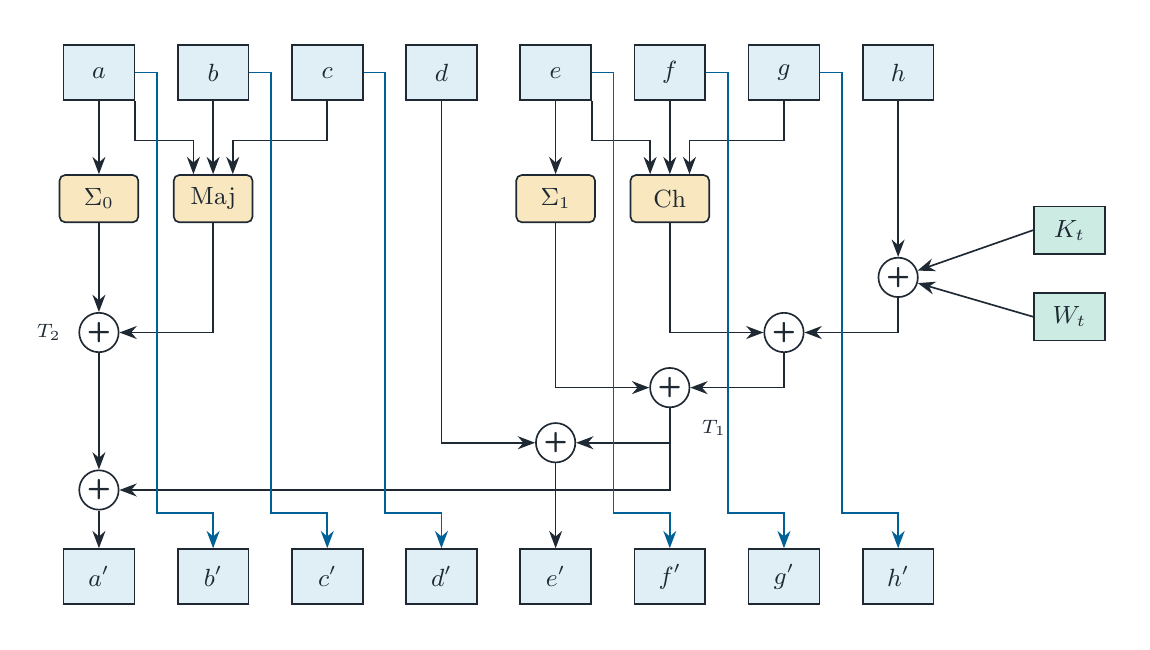
\begin{tikzpicture}
  \def\dx{1.45}
  % Working variables before and after the round.
  \foreach \v [count=\i from 0] in {a,b,c,d,e,f,g,h} {
    \node[reg] (in\v) at (\i*\dx, 0) {$\v$};
    \node[reg] (out\v) at (\i*\dx, -6.4) {$\v'$};
  }
  % The round functions.
  \node[fn] (S0) at (0, -1.6) {$\Sigma_0$};
  \node[fn] (maj) at (\dx, -1.6) {$\mathrm{Maj}$};
  \node[fn] (S1) at (4*\dx, -1.6) {$\Sigma_1$};
  \node[fn] (ch) at (5*\dx, -1.6) {$\mathrm{Ch}$};
  % The round inputs.
  \node[input] (K) at (8.5*\dx, -2.0) {$K_t$};
  \node[input] (W) at (8.5*\dx, -3.1) {$W_t$};
  % Additions modulo 2^w.
  \node[add] (t1a) at (7*\dx, -2.6) {+};
  \node[add] (t1b) at (6*\dx, -3.3) {+};
  \node[add] (t1)  at (5*\dx, -4.0) {+};
  \node[add] (enew) at (4*\dx, -4.7) {+};
  \node[add] (t2)  at (0, -3.3) {+};
  \node[add] (anew) at (0, -5.3) {+};
  % Inputs of the functions.
  \draw[wire] (ina) -- (S0);
  \draw[wire] (ina.south east) |- ++(0,-0.5) -| ([xshift=-2.5mm]maj.north);
  \draw[wire] (inb) -- (maj);
  \draw[wire] (inc.south) |- ++(0,-0.5) -| ([xshift=2.5mm]maj.north);
  \draw[wire] (ine) -- (S1);
  \draw[wire] (ine.south east) |- ++(0,-0.5) -| ([xshift=-2.5mm]ch.north);
  \draw[wire] (inf) -- (ch);
  \draw[wire] (ing.south) |- ++(0,-0.5) -| ([xshift=2.5mm]ch.north);
  % T1.
  \draw[wire] (inh) -- (t1a);
  \draw[wire] (K.west) -- (t1a);
  \draw[wire] (W.west) -- (t1a);
  \draw[wire] (t1a) |- (t1b);
  \draw[wire] (ch) |- (t1b);
  \draw[wire] (t1b) |- (t1);
  \draw[wire] (S1) |- (t1);
  \node[font=\sffamily\scriptsize, anchor=north west] at ([xshift=1mm,yshift=-1mm]t1.south east) {$T_1$};
  % T2.
  \draw[wire] (S0) -- (t2);
  \draw[wire] (maj) |- (t2);
  \node[font=\sffamily\scriptsize, anchor=east] at ([xshift=-1mm]t2.west) {$T_2$};
  % a' = T1 + T2 and e' = d + T1.
  \draw[wire] (t2) -- (anew);
  \draw[wire] (t1) |- (anew);
  \draw[wire] (t1) |- (enew);
  \draw[wire] (ind) |- (enew);
  \draw[wire] (anew) -- (outa);
  \draw[wire] (enew) -- (oute);
  % The other variables move one place: b' = a, c' = b, d' = c, f' = e, g' = f, h' = g.
  \foreach \src/\dst in {a/b, b/c, c/d, e/f, f/g, g/h} {
    \draw[wire, hsblue!85!black] (in\src.east) -- ++(0.275,0) coordinate (s)
      -- ($(s |- out\dst.north)+(0,0.45)$) -| (out\dst.north);
  }
  \begin{scope}[on background layer]
    \node[card, fit=(ina)(outh)(K)(W), inner sep=6pt] {};
  \end{scope}
\end{tikzpicture}
\end{document}
